\documentclass{report}
\usepackage{graphicx}
\usepackage{wrapfig}
\usepackage{enumerate}
\graphicspath{{./images/}}

\title{A VR Application Proposal: Spatial Learning Evaluation in a Virtual Reality Environment with SpatialLearningVR}
\author{by Nelson Jaimes}
\date{\today}

\begin{document}
\maketitle

\chapter*{Topics Map}
\section*{Introduction}
\begin{enumerate}[{1.}1]
  \item Project Goal
  \item Who is this for?
  \item Why is this important?
\end{enumerate}
\section*{VR App Design Overview}
\begin{enumerate}[{2.}1]
  \item Method Overview
  \item Feature List
\end{enumerate}
\section*{Development Platform}
\begin{enumerate}[{3.}1]
  \item Project Specifics
\end{enumerate}
\section*{Target VR Headset(s)}
\begin{enumerate}[{4.}1]
  \item Project Specifics
\end{enumerate}
\section*{Additional Features Considered}
\begin{enumerate}[{5.}1]
  \item Competitors and Product Inspiration
  \item Deliverables, Timeline and Deadlines
  \item User Personas
\end{enumerate}

\chapter*{Project Overview}

\section*{Project Name}
SpatialLearningVR

\section*{Project Goal}
This project aims to develop and test a tool that can be used to measure human spatial learning ability in a head mounted virtual reality (VR) environment. The tool can be used by experimenters in conjunction with surveys to measure spatial learning using different modalities.

\section*{Who is this for?}
Researchers that use the app as a tool to determine spatial learning ability will be able to use it in conjunction with surveys to determine the relationship between spatial learning ability in virtual reality and other factors, such as relationship to other mental abilities or neuronal dysfunction. Users (i.e. test subjects) of the spatial learning game will enjoy a fun challenge that tests their spatial learning ability.

\section*{Why is this important?}
Spatial ability has been linked to intelligence and creativity. For instance, individuals working in science, technology, engineering and math (STEM) have scored higher on spatial aptitude tests. In the brain, spatial learning ability has been linked with the hippocampus and surrounding areas. These brain regions are also damaged in early adulthood in individuals that are genetically predisposed with Alzheimer's Disease. Spatial ability has also been evaluated in relation to other diseases of the brain and nervous system. There are many measures of spatial learning ability in academic literature, including variations of the Morris Water Maze (MWM) and spatial learning scales like the The Visual Spatial Learning Test (VSLT). A low-cost behavioral test that can be run by anyone with an Oculus Quest headset can bridge the gap between surveys, costly virtual options, and in-person behavioral testing. Moreover, a test that can be run without the need for in-person interaction is currently more appealing given the current social constraints due to the latest pandemic.

\section*{Method Overview}
The Oculus Quest 2 will be used to deliver a test of spatial ability to human test subjects in VR. The data collected by the test of spatial ability can then be paired with other tests as determined by the researcher's goals and interests. For demonstration purposes, test subjects spatial ability scores will be collected in tandem with an electronic survey of self-reported spatial ability.

\section*{Feature List}

The SpatialLearningVR app will:
\begin{enumerate}
  \item use reward for finding objectives to provide motivation for test subjects as a substitute for the relief of removing water-related discomfort that rodents might feel in the MWM.
  \item train test subjects to use the interface by guiding audio and sound effects, text, and navigation features.
  \item be free to use at the time of release!
\end{enumerate}

The SpatialLearningVR app will calculate relevant measures of spatial learning ability such as:
\begin{enumerate}
  \item Time to reach visible objectives
  \item Time to reach unseen objectives
  \item Path length in reaching visible objectives
  \item Path length in reaching unseen objectives
  \item Time spent standing still
  \item Number of passes through area near objective
  \item Number of virtual steps (teleportations) to reach objective
  \item Accuracy in objective guess
\end{enumerate}

\section*{Competitors and Product Inspiration}
\begin{enumerate}
    \item HVS Image virtual reality MWM. A virtual reality test of learning ability that closely resembles the MWM task that is widely used in rodent spatial ability testing. It offers a range of different environments (e.g. rodent point of view and idealized point of view) and movement modalities (e.g. omni-directional treadmill and oculus thumbstick controls). A proxy for the discomfort or fear a mouse might experience as motivation to complete the MWM does not appear to be included in this tool. This tool appears to be expensive. https://hvsimage.com/virtual-reality/morris-water-maze/
    \item Conduct Science Virtual MWM. Another virtual reality test of learning ability that closely resembles the MWM task that is widely used in rodent spatial ability testing. It offers compatibility for a range of devices, including VR and computer-based interaction.  A proxy for the discomfort or fear a mouse might experience as motivation to complete the MWM does not appear to be included in this tool. This tool currently costs from 2190 to 5290 dollars. https://conductscience.com/maze/portfolio/virtual-reality-morris-water-maze/
\end{enumerate}

\section*{Deliverables}
\begin{enumerate}
  \item Project status update (including screenshots and video capture) of SpatialLearningVR app explaining the design and development process.
  \item SpatialLearningVR app for the Oculus Quest 2.
  \item Promotional video for app (2 minutes).
  \item App live presentation and live demonstration (5 minutes).
  \item Final 7-10 page report on the design and development process.
\end{enumerate}

\section*{Timeline and Deadlines}
\begin{enumerate}
  \item \textbf{February 10.} Project status, screenshots, and video capture of VR app explaining the design and development process.
  \item \textbf{February 24.} Published SpatialLearningVR app with a 2-minute promotional video.
  \item \textbf{Mar 3.} App live presentation and live demonstration (5 minutes). Final 7-10 page report.
\end{enumerate}

\chapter*{User Personas}

There are two different end-users for this tool. Researchers will use the tool to measure the spatial ability in human test subjects. Test subjects will use the tool to help researchers and to have fun.

\vspace{10mm}

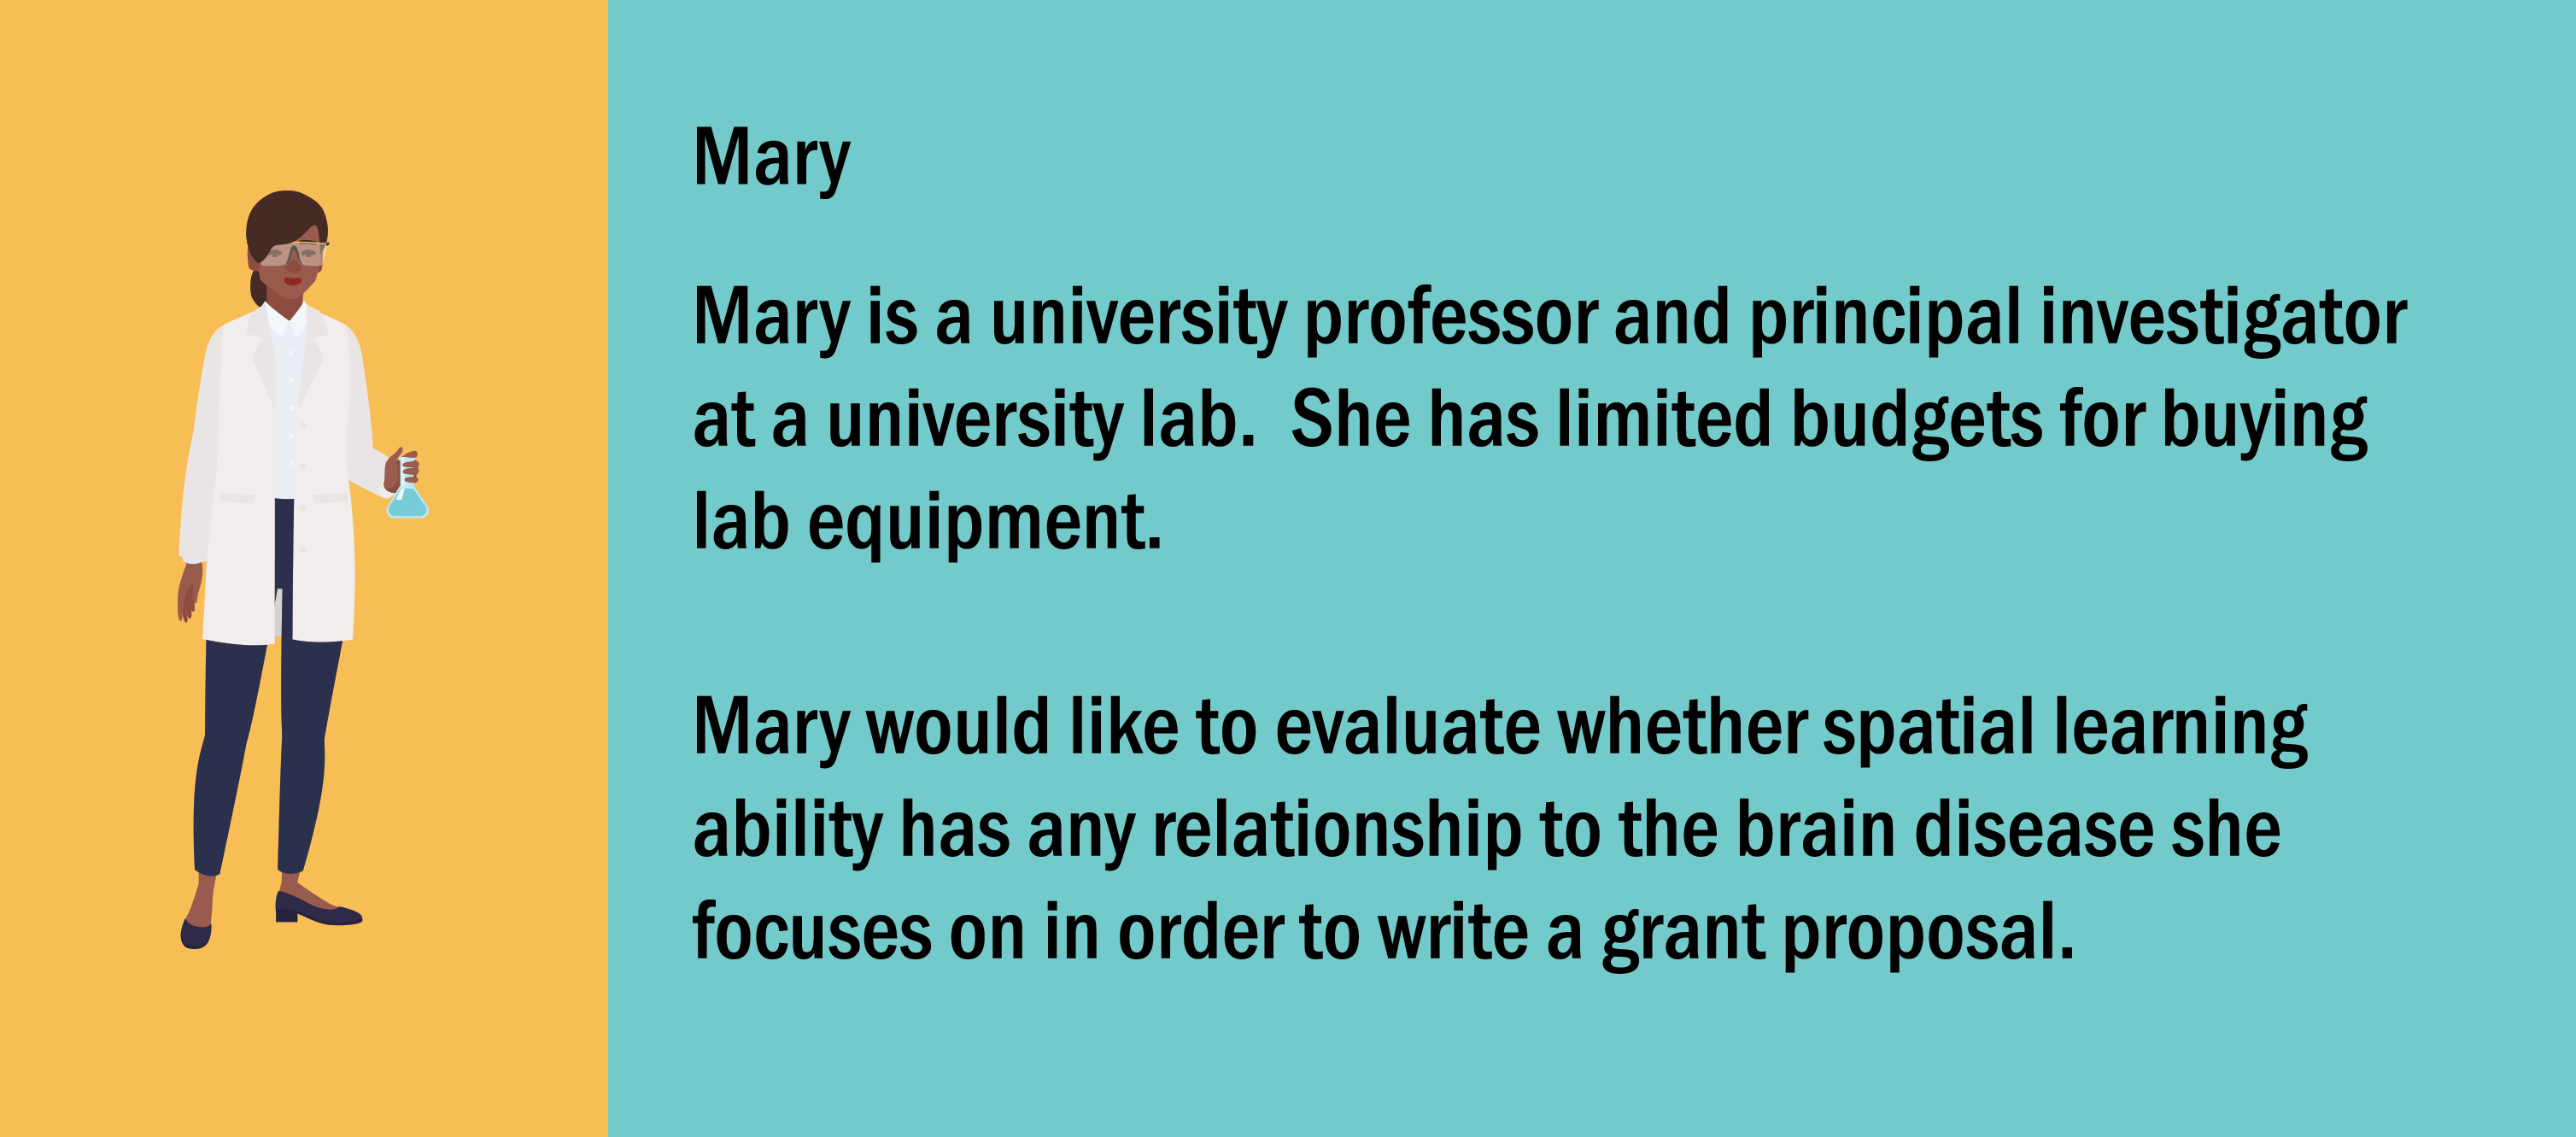
\includegraphics[width=1\textwidth]{Mary_with_story}

\vspace{10mm}

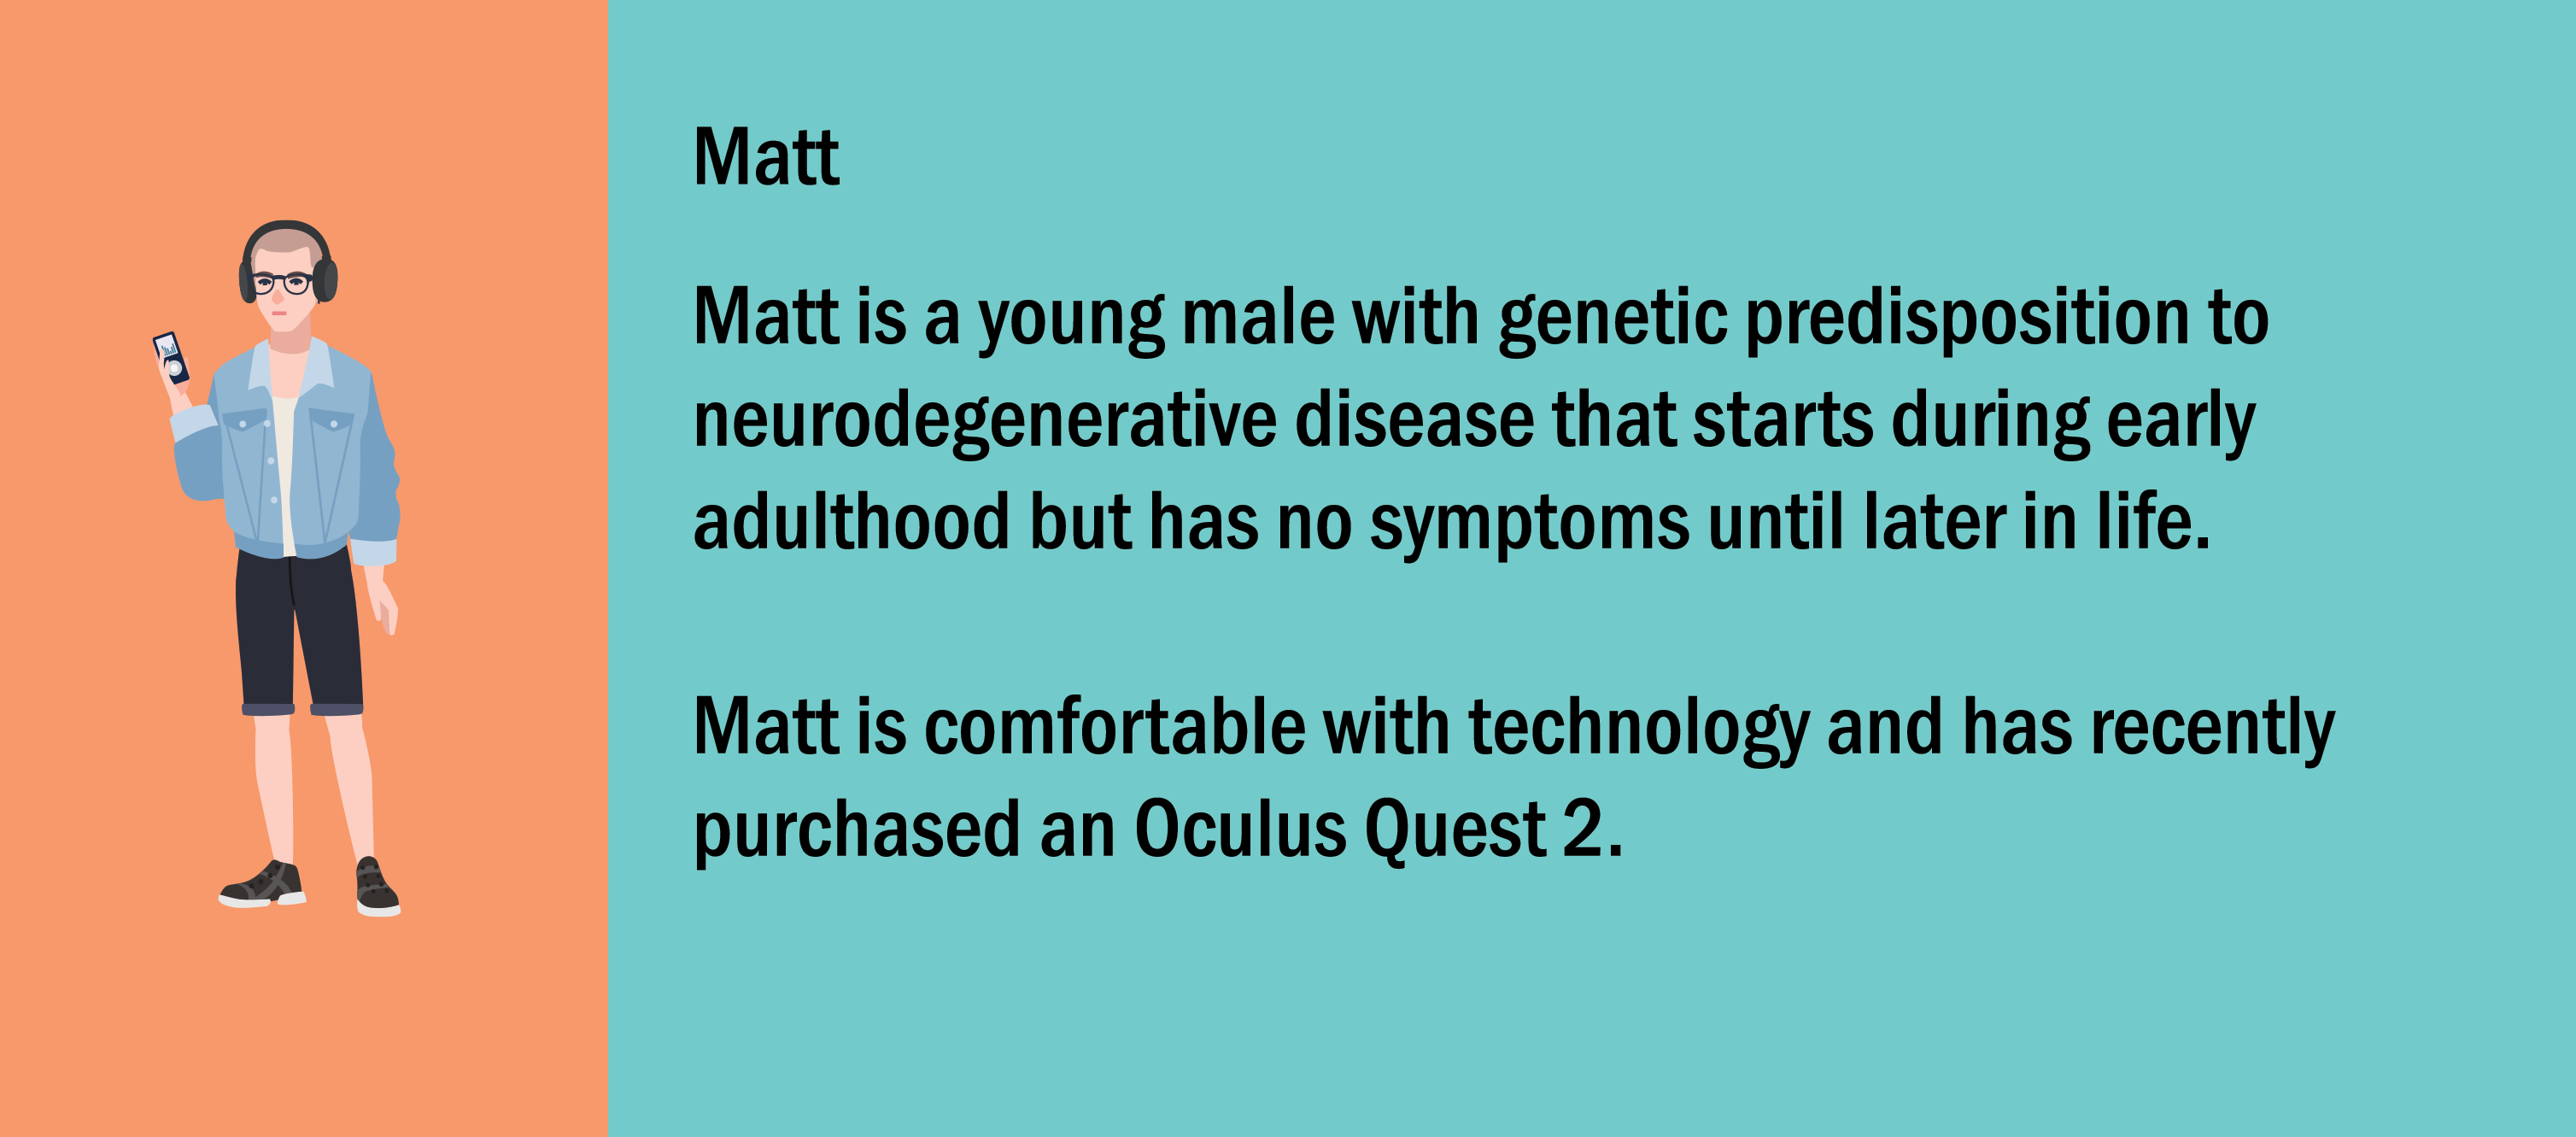
\includegraphics[width=1\textwidth]{Matt_with_story}

\chapter*{Project Specifics}
\section*{Development Platform}
This app will be developed on Windows 11.

\section*{Target VR Headset(s)}
This app will be targeted to the Oculus Quest 2.

\chapter*{Notes}
\begin{enumerate}
  \item This document aims to outline the upper boundary for functionality. The requirements outlined in the requirements document will be prioritized to ensure that deadlines are met, and any remaining work can be postponed for continued work.
  \item UX Analysis of this app will be included for project reports wherever possible given the project scope and time constraints.
  \item Stock images from Adobe Stock.
\end{enumerate}

\end{document} 